\documentclass[a4paper, 12pt]{article}

\usepackage[portuges]{babel}
\usepackage[utf8]{inputenc}
\usepackage{amsmath}
\usepackage{indentfirst}
\usepackage{graphicx}
\usepackage{multicol,lipsum}
\usepackage{listings}
\usepackage{graphicx}
\usepackage{float}
\usepackage[portuguese]{babel}

\begin{document}
%\maketitle

\begin{titlepage}
	\begin{center}
	
	%\begin{figure}[!ht]
	%\centering
	%\includegraphics[width=2cm]{c:/ufba.jpg}
	%\end{figure}

		\large{Centro Federal de Educação Tecnológica de Minas Gerais}\\
		\large{Departamento de Engenharia de Computação}\\ 
		\large{Sistemas Operacionais}\\ 
		\vspace{15pt}
        \vspace{95pt}
        \textbf{\LARGE{Adição de um módulo ao kernel}}\\
		%\title{{\large{Título}}}
		\vspace{3,5cm}
	\end{center}
	
	\begin{flushleft}
		\begin{tabbing}
			Aluno: Gabriel Siqueira Silva \\
			Professor: Bruno Santos \\
		\end{tabbing}
 \end{flushleft}
	\vspace{1cm}
	
	\begin{center}
		\vspace{\fill}
			 Agosto\\
		      2022
			\end{center}
\end{titlepage}
%%%%%%%%%%%%%%%%%%%%%%%%%%%%%%%%%%%%%%%%%%%%%%%%%%%%%%%%%%%

% % % % % % % % %FOLHA DE ROSTO % % % % % % % % % %

\begin{titlepage}
	\begin{center}
	
	%\begin{figure}[!ht]
	%\centering
	%\includegraphics[width=2cm]{c:/ufba.jpg}
	%\end{figure}

		\large{Centro Federal de Educação Tecnológica de Minas Gerais}\\
		\large{Departamento de Engenharia de Computação}\\ 
		\large{Sistemas Operacionais}\\ 
\vspace{15pt}
        
        \vspace{85pt}
        
		\textbf{\LARGE{Relatório}}
		\title{\large{Adição de um módulo ao kernel}}
	%	\large{Modelo\\
     %   		Validação do modelo clássico}
			
	\end{center}
\vspace{1,5cm}
	
	\begin{flushright}

   \begin{list}{}{
      \setlength{\leftmargin}{4.5cm}
      \setlength{\rightmargin}{0cm}
      \setlength{\labelwidth}{0pt}
      \setlength{\labelsep}{\leftmargin}}

      \item Primeiro Relatório de Sistema Operacional com o objetivo de entender o processo de alteração do kernel de uma distribuição Linux

      \begin{list}{}{
      \setlength{\leftmargin}{0cm}
      \setlength{\rightmargin}{0cm}
      \setlength{\labelwidth}{0pt}
      \setlength{\labelsep}{\leftmargin}}

			\item Aluno: Gabriel Siqueira \
            \item Professor: Bruno Santos \

      \end{list}
   \end{list}
\end{flushright}
\vspace{1cm}
\begin{center}
		\vspace{\fill}
		 Agosto\\
		 2022
			\end{center}
\end{titlepage}
\newpage
% % % % % % % % % % % % % % % % % % % % % % % % % %
\newpage
\tableofcontents
\thispagestyle{empty}

\newpage
\pagenumbering{arabic}
% % % % % % % % % % % % % % % % % % % % % % % % % % %
\section{Adição do módulo Hello World ao kernel}

\subsection{Procedimentos iniciais}
Para realizar esse trabalho prático utilizou-se o WSL2 na distribuição Ubuntu 20.04 que tem o kernel base 5.10.16.3-microsoft-standard-WSL2. O kernel modificado será a versão 5.15.y disponível no github da microsoft e para tal utilizou-se o git clone para utilizar o repositório. 

\begin{figure}[h]
\centering 
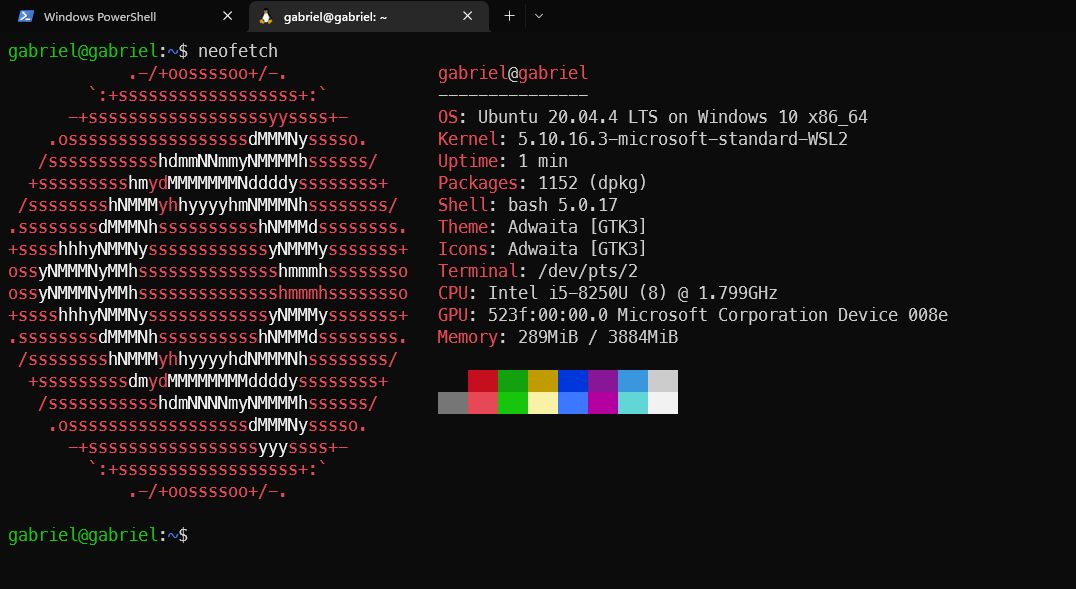
\includegraphics[width=13.5cm]{old_kernel.png}
\label{figura:qualquernome}
\caption{Kernel antigo}
\end{figure}

\subsection{Hello World}
O módulo adicionado será o Hello World e para isso cria-se um diretório dentro desse kernel com um código em c, como apresentado abaixo:

\begin{lstlisting} 
#include <linux/kernel.h>
#include <linux/syscalls.h>

SYSCALL_DEFINE0(hello)

{
    printk("Hello World.\n");
    return 0;
} 
\end{lstlisting}

\begin{figure}[h]
\centering 
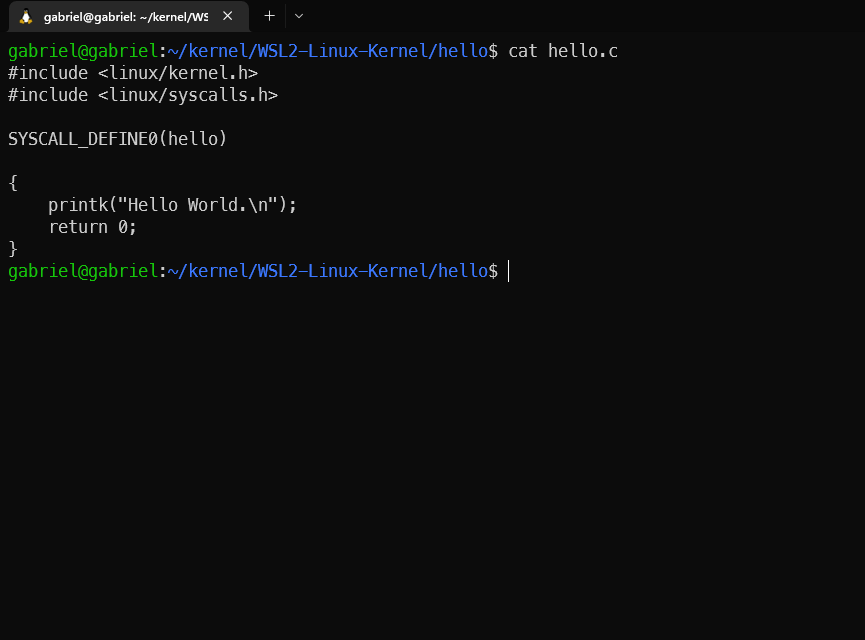
\includegraphics[width=13.5cm]{cat_hello.png}
\label{figura:qualquernome}
\caption{Código em C}
\end{figure}

Onde está o arquivo em c, deve-se criar um Makefile apresentando um arquivo objeto obtido após a compilação e além disso no Makefile do kernel deve-se mostrar quais são os módulos pertencentes ao mesmo e portanto é necessário alterar adicionando o hello aos módulos no core-y.

\begin{figure}[!htb]
\centering 
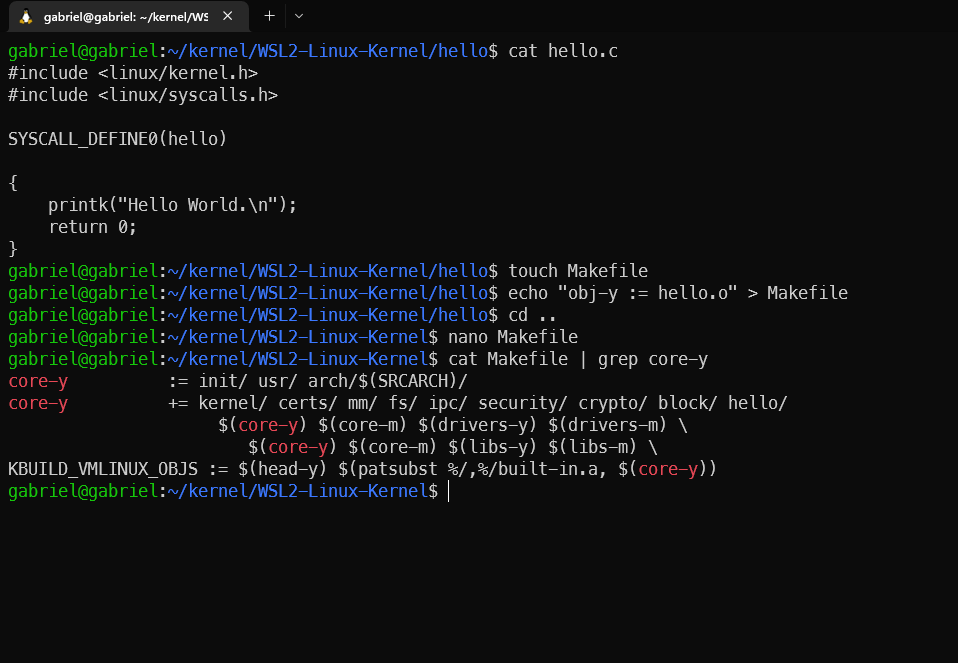
\includegraphics[width=13.5cm]{cat_mf.png}
\label{figura:qualquernome}
\caption{Makefile}
\end{figure}

\newpage

Agora, o hello deve ser conhecido como chamada de sistema e para isso no diretório de inclusão que tem o syscalls.h deve-se adicionar o
\begin{lstlisting} 
    asmlinkage long sys_hello(void) 
\end{lstlisting}  
e além disso, essa chamada deve ser adicionada na tabela de chamadas.

\newpage 

\begin{figure}[!h]
\centering 
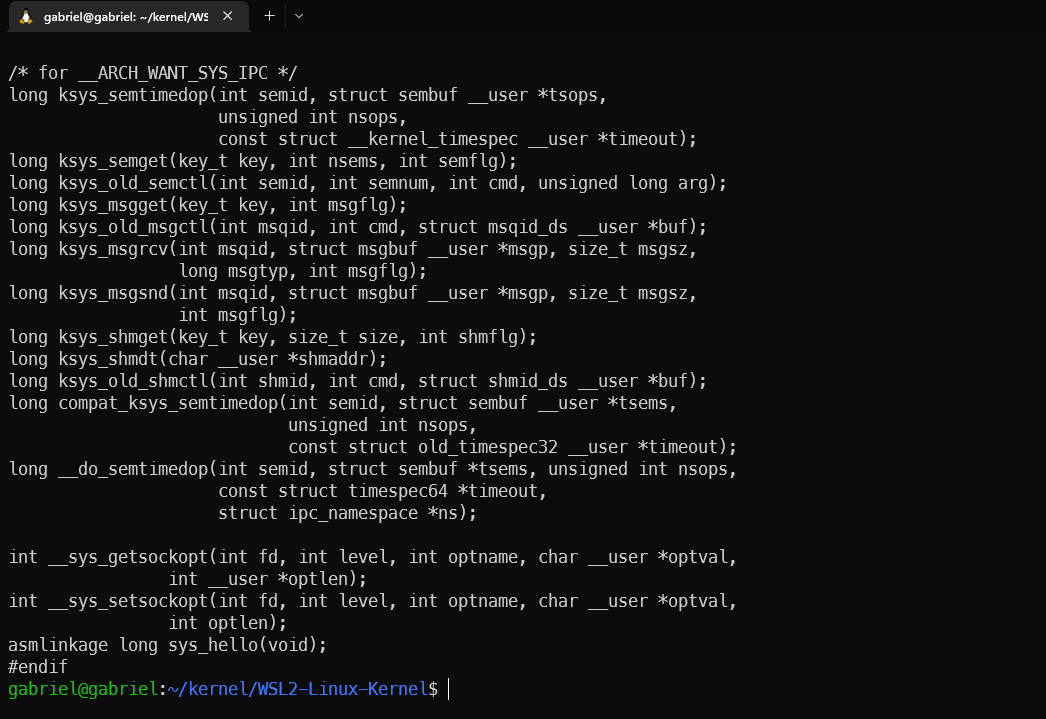
\includegraphics[width=13.5cm]{cat_syscalls_h.png}
\label{figura:qualquernome}
\caption{Chamadas}
\end{figure}

\begin{figure}[!h]
\centering 
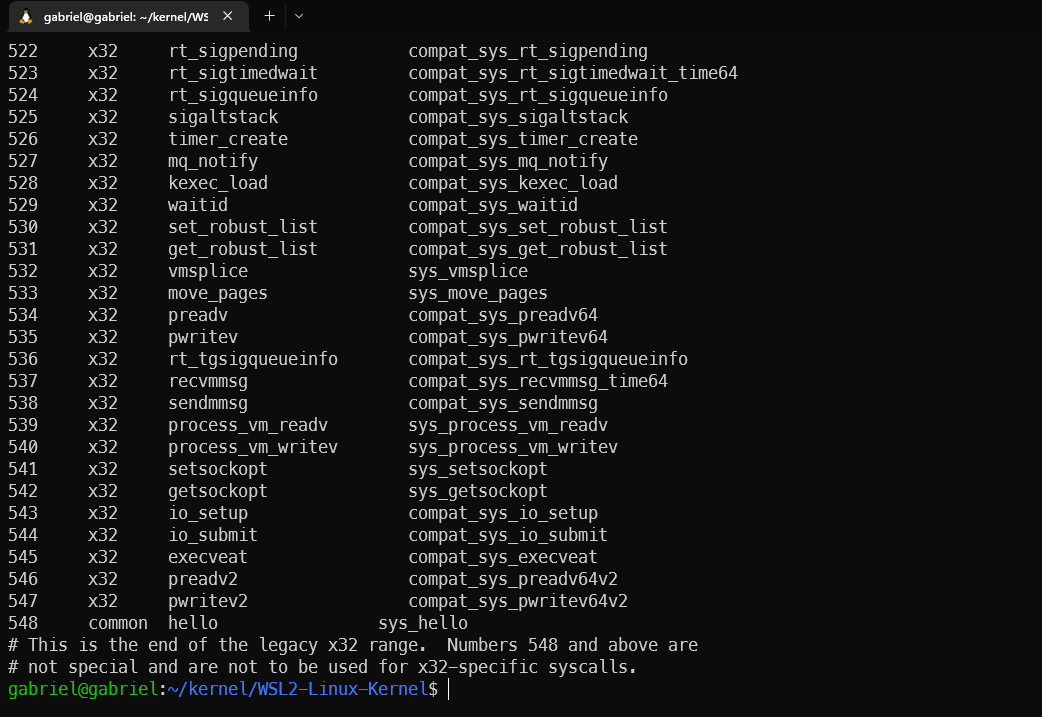
\includegraphics[width=13.5cm]{cat_table.png}
\label{figura:qualquernome}
\caption{Tabela}
\end{figure}

\newpage

\subsection{Compilação no WSL2}

Para complicar no wsl se usa 
\begin{lstlisting} 
    make KCONFIG_CONFIG=Microsoft/config-wsl 
\end{lstlisting} alterando o parâmetro j caso queira utilizar mais cores da sua máquina do que o padrão e o resultado final fica armazenado na pasta do kernel baixado com o nome vmlinux além do bzImage identificado na imagem.

\begin{figure}[!h]
\centering 
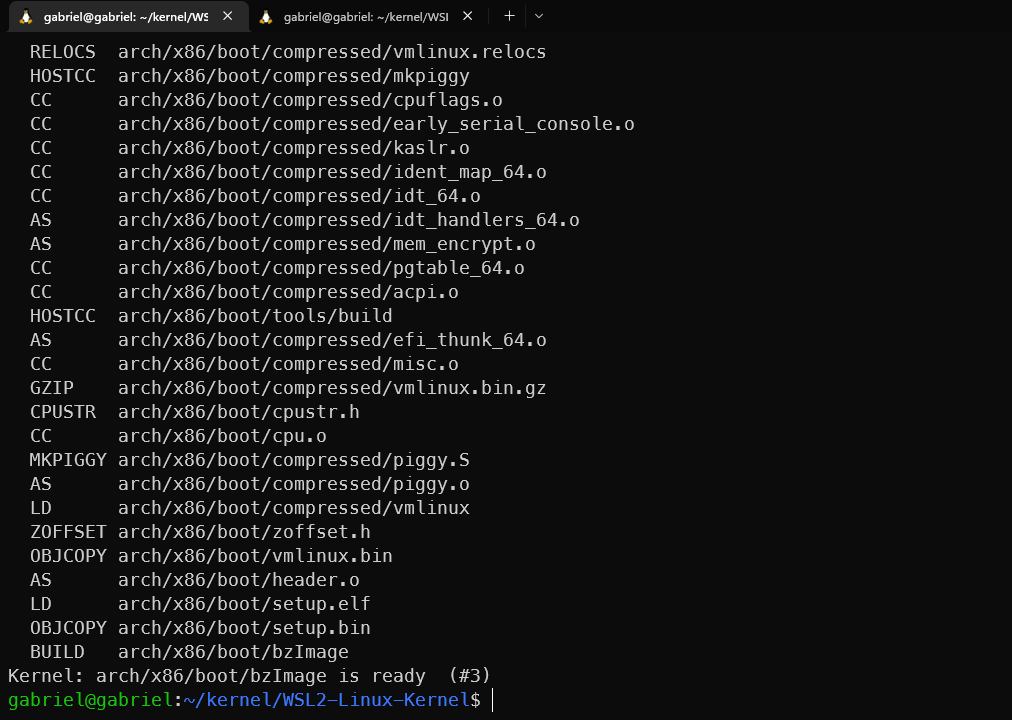
\includegraphics[width=13.5cm]{ready.png}
\label{figura:qualquernome}
\caption{Compilação terminada}
\end{figure}

\newpage

\subsection{Configuração}

Movendo o arquivo executável para o usuário no windows faremos com que a informação do kernel do linux presente no windows seja alterada pelo valor dessa vmlinux com o código:

\begin{lstlisting} 
    [wsl2]
    kernel=C:\\Users\\<Nome_Usuário>\\vmlinux 
\end{lstlisting}

Dessa forma o kernel muda como segue a imagem:

\newpage

\begin{figure}[!h]
\centering 
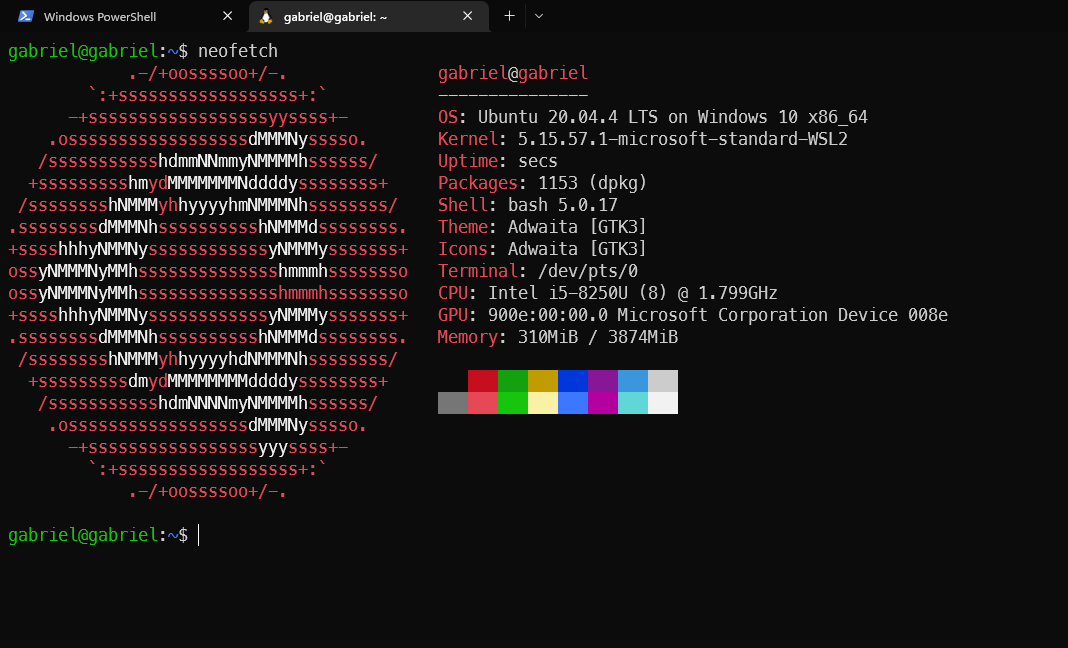
\includegraphics[width=13.5cm]{other-kernel.png}
\label{figura:qualquernome}
\caption{Kernel alterado}
\end{figure}

\subsection{Teste}

Compilando e executando o seguinte código em c obtemos uma chamada de sistema como a imagem posterior descreve.

\begin{lstlisting} 
#include <stdio.h>
#include <linux/kernel.h>
#include <sys/syscall.h>
#include <unistd.h>
int main()
{
         long int amma = syscall(548);
         printf("System call sys_hello returned %ld\n", amma);
         return 0;
}
\end{lstlisting}

\begin{figure}[!h]
\centering 
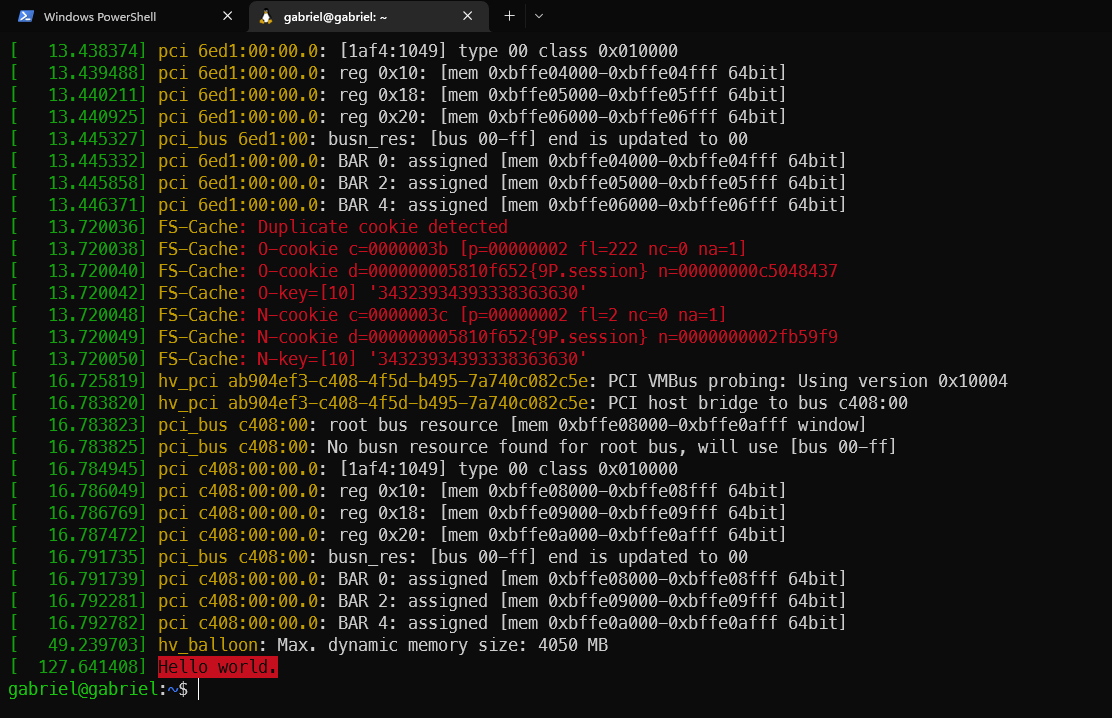
\includegraphics[width=13.5cm]{final.png}
\label{figura:qualquernome}
\caption{Resultado final}
\end{figure}

\newpage

\section{Questões}
\begin{enumerate}
		\item A implementação da chamada de sistema e o teste funcionaram corretamente? Em caso de negativo, explique o motivo.
		
		Resposta: Sim, funcionou.
		
		\item Qual é o nome do arquivo executável que corresponde ao Kernel?
		
		Resposta: O arquivo bzImage aparece como executável, bem como o vmlinux que também é gerado por esse procedimento.
		
		\item Após a instalação do Kernel, em qual local (diretório) foi armazenado o executável do Kernel?
		
		Resposta: Em 
		
		\item Em qual nível de privilégio a chamada de sistema implementada irá executar (usuário ou kernel/núcleo)?
		
		Resposta: 
		
		\item Um roteiro típico contendo as etapas da execução de uma chamada de sistema é apresentado nas páginas 23 e 24 do livro (Capítulo 2 do livro do Mazieiro). Você entendeu todos os passos de 1 a 8?
		
		\item 6.	O Kernel precisará de ser recompilado toda vez que uma nova funcionalidade for adicionada ao kernel? Explique. Provavelmente, você terá que pesquisar na internet. Não precisa se preocupar em dar a resposta correta, apenas pense sobre o assunto e procure responder a questão.
		
	\end{enumerate}
\newpage

\addcontentsline{toc}{section}{Bibliografia}
\section*{Bibliografia}
\footnotesize{

\noindent AGUIRRE, L. A. Introdução à Identificação de Sistemas, Técnicas Lineares e Não lineares Aplicadas a Sistemas Reais. Belo Horizonte, Brasil, EDUFMG. 2004.\\

}
\newpage
\end{document}



